%% ============================================================================
%% Restoration and Reliability: The Exact Moment Threshold for Controlling
%% Expansive Systems over Erasure Channels
%% Target: IEEE Transactions on Automatic Control (IEEEtran journal class).
%% Author names and affiliations intentionally left blank.
%% ============================================================================
\documentclass[journal]{IEEEtran}

\usepackage{amsmath,amssymb,amsfonts}
\usepackage{amsthm}
\usepackage{graphicx}
\usepackage{booktabs}
\usepackage{array}
\usepackage{tikz}
\usepackage{pgfplots}
\pgfplotsset{compat=1.18}
\usetikzlibrary{arrows.meta,positioning,calc,decorations.pathmorphing,backgrounds,shapes.geometric}
\usepackage[hidelinks]{hyperref}
\usepackage{cite}
\usepackage{xcolor}

\graphicspath{{../Figures/}}

\newtheorem{theorem}{Theorem}
\newtheorem{lemma}{Lemma}
\newtheorem{proposition}{Proposition}
\newtheorem{corollary}{Corollary}
\theoremstyle{definition}
\newtheorem{definition}{Definition}
\newtheorem{assumption}{Assumption}
\theoremstyle{remark}
\newtheorem{remark}{Remark}

\newcommand{\rvol}{r^\star_{\mathrm{vol}}}
\newcommand{\rtop}{r^\star_{\mathrm{top}}}
\newcommand{\hR}{h_R}
\newcommand{\ach}{\alpha_{\mathrm{ch}}}
\newcommand{\R}{\mathbb{R}}
\newcommand{\E}{\mathbb{E}}
\newcommand{\dplus}{d^{+}}
\DeclareMathOperator{\diam}{diam}
\DeclareMathOperator{\Vol}{Vol}
\DeclareMathOperator*{\limsupop}{lim\,sup}

\begin{document}

\title{Restoration and Reliability: The Exact Moment\\ Threshold for Controlling Expansive Systems\\ over Erasure Channels}

\author{\thanks{Manuscript submitted for review. This work is intended for the IEEE Transactions on Automatic Control.}}

\markboth{IEEE Transactions on Automatic Control}%
{Restoration and Reliability: Controlling Expansive Systems over Erasure Channels}

\maketitle

\begin{abstract}
An unstable process whose state expands on its own must be kept inside a valid region while it is controlled over
a link that drops packets at random. We determine the exact condition under which the estimation error stays
bounded in the sense of its $m$-th moment, for a general continuously differentiable expansive map over a
memoryless erasure channel. The condition is a single number below one, and it splits into two independent
requirements. The first is a bandwidth requirement, in which the average delivered rate must exceed the
restoration entropy of the map. The second is a reliability requirement, in which the erasure probability times
the $m$-th power of the top expansion factor must stay below one. We prove that both are necessary, and we prove
a matching achievability using a universal zooming quantizer that reaches the exact threshold without any
quasi-conformality assumption, so necessity and sufficiency meet with no gap. We confirm the result with
rare-event importance sampling on two analytically solvable surrogates and on non-normal and non-uniform stress
systems, recovering the predicted threshold surface to within a few thousandths of a nat.
\end{abstract}

\begin{IEEEkeywords}
Networked control, quantized control, data-rate theorem, erasure channel, restoration entropy, anytime capacity,
nonlinear observation, moment stability.
\end{IEEEkeywords}

%% ===========================================================================
\section{Introduction}
%% ===========================================================================
\IEEEPARstart{M}{any} modern control loops are closed over a shared network rather than a dedicated wire. The
plant sends its measurements as packets, some of which are lost, and the controller must still keep the plant
inside a safe region. When the plant is unstable the difficulty is sharp, because the estimation error grows on
its own between useful updates, and a run of dropped packets can let it grow beyond recovery. The question we
answer is how much communication, in both average rate and reliability, is needed to keep the error bounded in
the sense of its $m$-th moment.

The classical theory answers this only when the obstacles are separated. Over a noiseless finite-rate link a
linear plant is mean-square stabilizable exactly when the rate exceeds the sum of the unstable logarithmic
eigenvalues, which is the data-rate theorem of Tatikonda and Mitter and of Nair and Evans
\cite{tatikondamitter2004,nairevans2004}. For a nonlinear plant the minimal rate for set-invariance over a
noiseless link is the topological feedback entropy \cite{nemm2004}. When the link instead drops packets at
random, the linear theory gives a reliability threshold, in which the erasure probability times the squared gain
must stay below one \cite{sinopoli2004,elia2005}, and the anytime-capacity theory of Sahai and Mitter shows that
a reliability exponent above $m$ times the log-gain is needed for $m$-th-moment stability \cite{sahaimitter2006}.
What has been missing is the exact condition when the plant is a general nonlinear expansive map and the channel
drops packets at random, so that the bandwidth obstacle and the reliability obstacle are present together and
must both be met.

This paper settles that case. Let $\hR$ be the restoration entropy of the map on the target set, a worst-case
rate at which the map creates volume, let $\rtop$ be the top expansion rate, the fastest rate at which a single
direction stretches, and let $p$ be the erasure probability. Our main result is that the error is $m$-th-moment
bounded if and only if a single per-step multiplier stays below one,
\begin{equation}
\gamma \;=\; (1-p)\,e^{m(\hR-R)/\dplus} \;+\; p\,e^{m\rtop} \;<\; 1, \label{eq:gamma}
\end{equation}
where $R$ is the per-packet rate and $\dplus$ is the number of expanding directions. The first term is the effect
of a delivered packet, which contracts the error, and the second is the effect of an erasure, which lets it
expand. The two marginal projections of \eqref{eq:gamma} are a rate condition and a reliability condition that we
write as
\begin{align}
\text{(R)}\quad & R\,(1-p)\ \ge\ \hR, \label{eq:R}\\
\text{(A)}\quad & p\,e^{m\rtop}\ <\ 1. \label{eq:A}
\end{align}

Our contributions are the following. We first prove, in Theorem~\ref{thm:nec}, that both conditions are necessary
for every causal coder and controller, with or without acknowledgment, because erasure bursts expand the error
uniformly and recur without bound. We then prove, in Theorem~\ref{thm:ach}, a matching achievability at the exact
surface \eqref{eq:gamma} using a universal zooming quantizer whose partition is driven by the shared index
history rather than the unknown state, which removes the difficulty that the grid would otherwise depend on where
the plant is. The two results meet with no gap and with no quasi-conformality assumption. We show that the rate
requirement is set by the volume rate while the reliability requirement is set by the top rate, so a plant with
several unstable directions is governed by two different numbers. Finally we validate every part of the theory
with an exact rare-event estimator on analytically solvable surrogates and on stress systems that scalar or
normal surrogates cannot probe.

Section~\ref{sec:model} sets up the model. Section~\ref{sec:related} places the result among six strands of prior
work. Section~\ref{sec:results} states the theorems. Sections~\ref{sec:nec} and \ref{sec:ach} prove necessity and
achievability. Section~\ref{sec:surr} gives the surrogates and the estimator. Section~\ref{sec:exp} reports the
experiments. Sections~\ref{sec:disc} and \ref{sec:conc} discuss limitations and conclude.

%% ===========================================================================
\section{Problem Formulation}\label{sec:model}
%% ===========================================================================
The plant is a discrete-time controlled system $x_{t+1}=f(x_t,u_t)$ on a compact region $K$ of a state space of
dimension $n$. Under ideal full-state feedback there is a control law that keeps a compact target set $Q\subseteq
K$ invariant, and we write $f$ for the resulting closed-loop map, assumed continuously differentiable on $K$.
Table~\ref{tab:notation2} collects the notation. The Jacobian $Df(x)$ has singular values $\sigma_1(x)\ge\cdots
\ge\sigma_n(x)$ in a chosen Riemannian metric, and the two expansion rates that matter are the volume rate and
the top rate,
\begin{equation}
\rvol=\inf_g\sup_{x\in K}\sum_{i}\log^{+}\sigma_i(x),\quad
\rtop=\inf_g\sup_{x\in K}\log^{+}\sigma_1(x), \label{eq:rates}
\end{equation}
where $\log^{+}=\max(0,\log)$ and the infimum is over Riemannian metrics. The volume rate sums the expansion over
all growing directions, while the top rate keeps only the fastest one, so $\rtop\le\rvol$ always, with equality
for scalar systems and for the two surrogates used later. For a linear map $Ax$ the top rate is the logarithm of
the spectral radius $\rho(A)$, and the infimum over metrics is what tightens the naive operator norm down to the
spectral radius.

\begin{table}[t]
\centering
\caption{Principal notation.}
\label{tab:notation2}
\renewcommand{\arraystretch}{1.25}
\begin{tabular}{@{}ll@{}}
\toprule
Symbol & Meaning \\
\midrule
$f,\ K,\ Q$ & closed-loop map, region, invariant target set \\
$Df(x),\ \sigma_i(x)$ & Jacobian and its singular values \\
$\rvol,\ \rtop$ & volume and top expansion rates \\
$\hR$ & restoration entropy of $f|_Q$, $\hR\le\rvol$ \\
$\dplus$ & number of expanding directions \\
$p$ & erasure probability, i.i.d. per use \\
$R$ & rate delivered per non-erased use (nats) \\
$e_t$ & observer estimation error at time $t$ \\
$m$ & moment order, $m\ge1$ \\
$\ach$ & anytime reliability exponent $\ln(1/p)$ \\
$\gamma$ & per-step $m$-th-moment multiplier \eqref{eq:gamma} \\
\bottomrule
\end{tabular}
\end{table}

The restoration entropy $\hR$ of Matveev and Pogromsky is the smallest rate at which a coder and observer can hold
the estimation error uniformly small against the worst initial error and bounded disturbance
\cite{matveevpogromsky2019}. It obeys $\hR\le\rvol$ and equals $\rvol$ when the map is uniformly quasi-conformal.
The key contrast with topological or Lyapunov entropy is that restoration entropy takes a supremum over the
region rather than an average along typical orbits, which is exactly what a worst-case burst bound needs. The
channel is a memoryless erasure channel that delivers $R$ nats with probability $1-p$ and erases with probability
$p$, independently across uses. The anytime reliability exponent of this channel is $\ach=\ln(1/p)$, because a
blackout of length $b$ has probability $p^{b}=e^{-b\ach}$. Figure~\ref{fig:model2} shows the loop. The property we
characterize is $m$-th-moment controlled set-invariance, meaning $\limsup_{t\to\infty}\E\,e_t^{m}<\infty$, and we
ask for the exact set of rates and erasure probabilities that achieve it.

\begin{figure}[t]
\centering
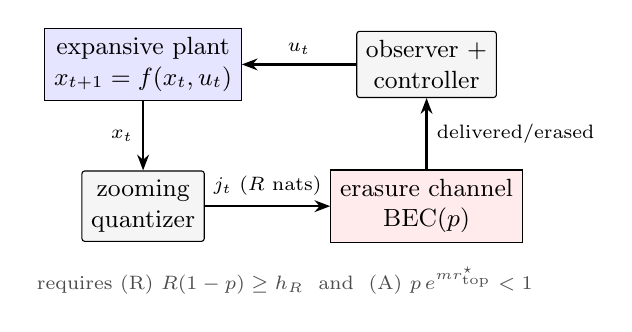
\begin{tikzpicture}[
  >={Stealth[length=2mm]},
  block/.style={draw,rounded corners=1pt,minimum height=7mm,minimum width=13mm,font=\small,align=center},
  plant/.style={draw,fill=blue!10,minimum height=8mm,minimum width=15mm,font=\small,align=center},
  chan/.style={draw,fill=red!8,minimum height=8mm,minimum width=15mm,font=\small,align=center},
  every node/.style={font=\small}]
  \node[plant] (P) at (0,0) {expansive plant\\ $x_{t+1}=f(x_t,u_t)$};
  \node[block,fill=black!4] (Q) at (0,-1.8) {zooming\\ quantizer};
  \node[chan] (C) at (3.6,-1.8) {erasure channel\\ $\mathrm{BEC}(p)$};
  \node[block,fill=black!4] (D) at (3.6,0) {observer +\\ controller};
  \draw[->,thick] (P.south) -- node[left,font=\scriptsize]{$x_t$} (Q.north);
  \draw[->,thick] (Q.east) -- node[above,font=\scriptsize]{$j_t$ ($R$ nats)} (C.west);
  \draw[->,thick] (C.north) -- node[right,font=\scriptsize]{delivered/erased} (D.south);
  \draw[->,thick] (D.west) -- node[above,font=\scriptsize]{$u_t$} (P.east);
  \node[align=center,font=\scriptsize,gray!60!black] at (1.8,-2.75)
     {requires (R) $R(1-p)\ge h_R$\ \ and\ \ (A) $p\,e^{m r^\star_{\mathrm{top}}}<1$};
\end{tikzpicture}
\caption{Control of an expansive plant over a memoryless erasure channel. The zooming quantizer sends an index
$j_t$ of $R$ nats, delivered with probability $1-p$ and erased with probability $p$. Bounded $m$-th-moment error
requires enough average rate to cover the restoration entropy and enough burst reliability to survive runs of
erasures.}
\label{fig:model2}
\end{figure}

%% ===========================================================================
\section{Related Work}\label{sec:related}
%% ===========================================================================
The result meets six strands of prior work, and it is best understood as the row that none of them fills.

The first strand is the data-rate theorem for a deterministic channel. Quantized stabilization and the tightest
rate bounds for linear plants \cite{wongbrockett1999,nairevans2000,brockettliberzon2000,delchamps1990,fuxie2005},
the mean-square data-rate theorem \cite{tatikondamitter2004,nairevans2004}, and the topological feedback entropy
for nonlinear set-invariance \cite{nemm2004} all assume no packet loss. They give the bandwidth requirement in
the noiseless case, and the present rate condition reduces to the data-rate theorem when the erasure probability
is zero. Broad overviews frame this program \cite{nair2007overview,matveevsavkin2009,yukselbasar2013}.

The second strand studies packet loss for linear plants. Kalman filtering with intermittent observations gives a
critical arrival probability \cite{sinopoli2004}, remote stabilization over fading and erasure links gives the
squared-gain reliability threshold \cite{elia2005,gupta2007}, and the minimum-rate results over lossy and Markov
channels give a spectral-radius condition on a modulated matrix together with a rate condition
\cite{youxie2010,minero2009,coviello2013}. These are the linear specializations that our reliability condition
recovers, and the modulated spectral radius reappears in our correlated-loss discussion. Surveys collect the
networked setting \cite{schenato2007,hespanha2007}.

The third strand is anytime capacity. The necessity and sufficiency of anytime capacity for stabilizing a linear
plant over a noisy link \cite{sahaimitter2006}, its stochastic-control companions
\cite{tsm2004,simsek2004,freudenberg2010,martins2006}, and explicit anytime and real-valued reliable codes
\cite{sukhavasi2016,como2010} give the reliability layer. The anytime exponent that a code must meet is exactly
the erasure-burst tail that drives our moment divergence, and the tree code is the transport layer of our
achievability. The linear anytime exponent uses a constant gain, which is ill-defined for a state-dependent
Jacobian, and we replace it by the uniform top rate.

The fourth strand is entropy for nonlinear control. Invariance entropy and its relatives
\cite{coloniuskawan2009,colonius2012,kawan2013,kawan2018,savkin2006,pogromsky2011} give the minimal rate for
set-invariance and exponential stabilization over a deterministic channel. Restoration entropy and its tight
singular-value estimates \cite{matveevpogromsky2016,matveevpogromsky2019} give the robust rate that survives
erasure, and fundamental limits for nonlinear observation over an erasure channel and a nonstochastic information
theory for estimation \cite{diwadkarvaidya2013,nair2013} are the closest in spirit. Our contribution over these
is the exact $m$-th-moment threshold surface with a matching zooming-quantizer achievability that needs no
quasi-conformality.

The fifth strand is nonlinear and predictive control under loss. Data-rate conditions for nonlinear quantized
stabilization \cite{liberzonhespanha2005,baillieul2004,liberzonnair2007,baillieulantsaklis2007} and input-to-state
stability of packetized predictive control under Markov drops \cite{quevedonesic2012} give sufficient conditions,
whereas we give the tight necessity in terms of an intrinsic entropy. The sixth strand supplies the mathematical
foundations, namely the singular-value and volume-growth machinery
\cite{katokhasselblatt1995,walters1982,pesin1977,oseledets1968}, products of random matrices and Markov jump
systems \cite{furstenbergkesten1960,costafragoso2005,fangloparo2002}, the burst-noise channel
\cite{gilbert1960,elliott1963}, the geometric-drift criterion \cite{meyntweedie2009}, and the channel-capacity
facts \cite{shannon1948,coverthomas2006d2,yuksel2010,kawan2018lyap}.

%% ===========================================================================
\section{Main Results}\label{sec:results}
%% ===========================================================================
We first give the intuition and then the formal statements. Track the error over one step. A delivered packet of
rate $R$ shrinks a $\dplus$-dimensional uncertainty by a factor $e^{(\hR-R)/\dplus}$, while an erasure lets the
error grow by the top expansion factor $e^{\rtop}$. Averaging the $m$-th power of these two outcomes over the
erasure coin gives the multiplier $\gamma$ of \eqref{eq:gamma}, and the error is bounded exactly when
$\gamma<1$. The rate condition and the reliability condition are the two edges of this surface, obtained by
sending the erasure probability to zero and the rate to infinity respectively.

\begin{theorem}[Necessity]\label{thm:nec}
Let $f$ be continuously differentiable and expansive on a compact $K$, let $Q$ be an invariant target, and let
the channel be a memoryless erasure channel with $p\in(0,1)$. Then $m$-th-moment controlled set-invariance
requires both the rate condition \eqref{eq:R} and the reliability condition \eqref{eq:A}, for every causal coder,
quantizer, and controller, with or without acknowledgment. If \eqref{eq:A} fails then
$\limsup_{t}\E\,e_t^{m}=\infty$ and escape from any fixed neighborhood of $Q$ occurs with probability one.
\end{theorem}

\begin{theorem}[Achievability]\label{thm:ach}
For every continuously differentiable expansive $f$ on a compact $K$, the universal zooming quantizer combined
with an anytime code achieves $m$-th-moment controlled set-invariance if and only if $\gamma<1$, that is
\begin{equation}
(1-p)\,e^{m(\hR-R)/\dplus}+p\,e^{m\rtop}\;<\;1. \label{eq:exact}
\end{equation}
The threshold is exact, with no back-off and no quasi-conformality assumption, and its marginals are the rate
condition \eqref{eq:R} and the reliability condition \eqref{eq:A}. As the erasure probability tends to zero the
critical rate tends to exactly $\hR$.
\end{theorem}

\begin{corollary}[Zero gap]\label{cor:zerogap2}
For a general continuously differentiable expansive map over a memoryless erasure channel, the necessity of
Theorem~\ref{thm:nec} and the achievability of Theorem~\ref{thm:ach} meet at the exact surface $\gamma=1$, so the
$m$-th-moment stabilizable region is determined with no gap.
\end{corollary}

The two conditions are genuinely independent, which is the structural advance over prior work where only one of
them appears. If the rate is very large but the erasure probability exceeds the reliability threshold, condition
\eqref{eq:A} fails and the moment diverges. If the erasure probability is tiny but the rate is below the
restoration entropy, condition \eqref{eq:R} fails and the error grows almost surely. Neither implies the other.
The linear case is a mandatory check that the theorem passes. For a scalar plant with gain $\lambda$ the two
rates coincide at $\ln|\lambda|$, the rate condition at zero erasure becomes $R\ge\ln|\lambda|$, which is the
data-rate theorem, and the reliability condition at $m=2$ becomes $p\,\lambda^{2}<1$, which is the intermittent
Kalman and remote-stabilization threshold \cite{tatikondamitter2004,sinopoli2004,elia2005}.

Two rates rather than one govern a vector plant, which scalar surrogates cannot reveal. The bandwidth requirement
uses the volume rate, because every expanding direction must be encoded, while the reliability requirement uses
the top rate, because the worst burst stretches the fastest direction. Table~\ref{tab:novelty2} places the result
against the prior art.

\begin{table*}[t]
\centering
\caption{Where the result sits. A check marks a feature that the row treats.}
\label{tab:novelty2}
\renewcommand{\arraystretch}{1.2}
\small
\begin{tabular}{@{}lccccc@{}}
\toprule
Work & nonlinear & random loss & $m$-th moment & restoration & achiev. \\
\midrule
Tatikonda-Mitter \cite{tatikondamitter2004} & & & MS & & \checkmark \\
Nair-Evans et al. \cite{nemm2004} & \checkmark & & set-inv. & TFE & \checkmark \\
Sinopoli, Elia \cite{sinopoli2004,elia2005} & & \checkmark & MS & & \checkmark \\
You-Xie \cite{youxie2010} & & Markov & MS & & \checkmark \\
Sahai-Mitter \cite{sahaimitter2006} & & \checkmark & $m$-th & & \checkmark \\
Matveev-Pogromsky \cite{matveevpogromsky2019} & \checkmark & & set-inv. & \checkmark & \checkmark \\
This paper & \checkmark & \checkmark & \checkmark & \checkmark & \checkmark \\
\bottomrule
\end{tabular}
\end{table*}

%% ===========================================================================
\section{Proof of Necessity}\label{sec:nec}
%% ===========================================================================
The strategy has three steps. We first show that an erasure burst expands the error uniformly at the top rate. We
then sum the moment contributions of the recurring bursts and find that the sum diverges exactly when the
reliability condition fails, and we show that acknowledgment cannot prevent this. We finally show that the average
rate must cover the restoration entropy, by the law of large numbers applied to the delivered packets.

\begin{lemma}[Uniform burst expansion]\label{lem:burst}
During an erasure burst of length $b$, in which no control information is delivered, the observer uncertainty set
$\mathcal U$ obeys $\diam f^{b}(\mathcal U)\ge\diam(\mathcal U)\,e^{b\rtop(1-o(1))}$ and $\Vol f^{b}(\mathcal U)\ge
\Vol(\mathcal U)\,e^{b\rvol(1-o(1))}$, uniformly over the location of $\mathcal U$ in $K$.
\end{lemma}

\begin{proof}
By the change-of-variables formula the volume of the image is the integral of the Jacobian determinant, and on
the expanding part $|\det Df(x)|\ge e^{\sum_i\log^{+}\sigma_i(x)}$. Taking the metric that attains the infimum in
\eqref{eq:rates}, the exponent is at most $\rvol$ with the supremum over $K$ attained, so the product over the
burst is at least $e^{b\rvol(1-o(1))}$ regardless of the orbit. This uniformity is the crux, and it holds because
the rate is a supremum over the region rather than an average along an orbit. For the diameter, two points of
$\mathcal U$ separated along the top singular direction have images that separate by the product of the top
singular values, which is at least $e^{b\rtop(1-o(1))}$. The sub-exponential factor is zero for uniformly
hyperbolic maps and does not affect the threshold in the next lemma, because a ratio test at ratio
$p\,e^{m\rtop}$ is unchanged by factors that grow slower than any exponential \cite{katokhasselblatt1995}.
\end{proof}

\begin{lemma}[Renewal moment divergence]\label{lem:renewal}
If $p\,e^{m\rtop}\ge1$ then $\limsup_{t}\E\,e_t^{m}=\infty$ for every causal scheme, with or without
acknowledgment.
\end{lemma}

\begin{proof}
In i.i.d. erasure the length of a run of consecutive erasures is geometric, with $\Pr[\text{run}=b]=(1-p)p^{b}$,
and runs recur infinitely often almost surely. At the start of a burst the error is at least the quantizer floor,
which is positive at any finite rate, and by Lemma~\ref{lem:burst} a burst of length $b$ inflates it to at least
that floor times $e^{b\rtop(1-o(1))}$. The $m$-th-moment contribution of such a burst is therefore at least a
constant times $e^{m\rtop b(1-o(1))}(1-p)p^{b}$, and summing over $b$ gives a series whose ratio is
$p\,e^{m\rtop}$, which diverges exactly when this ratio is at least one. A finite between-burst contraction cannot
save a series whose divergence is driven by its heavy tail at large $b$. Acknowledgment does not change this.
Future erasures are independent of the past, so a burst cannot be foreseen and the error cannot be pre-shrunk
below the floor, and by the Borel-Cantelli lemma runs longer than any fixed length occur infinitely often, so the
per-occurrence contribution is unbounded infinitely often \cite{sahaimitter2006,shannon1948}.
\end{proof}

\begin{lemma}[Rate necessity]\label{lem:rate}
If $R(1-p)<\hR$ then $\limsup_{t}\E\,e_t^{m}=\infty$, and escape from any neighborhood of $Q$ occurs almost
surely.
\end{lemma}

\begin{proof}
Over $n$ steps the number of delivered nats is $R$ times a binomial count of delivered packets, which by the
strong law of large numbers is almost surely $R(1-p)n$ to first order. Apply the volume-counting necessity of the
restoration-entropy theory to the realized delivery sequence \cite{matveevpogromsky2019}. Over $n$ steps the
observer receives at most this many nats, while the uncertainty volume grows by at least $e^{n\rvol(1-o(1))}$ by
the volume branch of Lemma~\ref{lem:burst}, so maintaining a bounded volume requires at least $n\hR(1-o(1))$ nats.
If the delivered count is below this, the volume is unbounded and the error diverges almost surely, and by
Fatou's lemma the $m$-th moment diverges as well. The substitution of the average rate $R(1-p)$ for $R$ is exact
almost surely rather than an approximation, because the counting argument is deterministic given the realized
pattern and the law of large numbers fixes the count.
\end{proof}

Theorem~\ref{thm:nec} follows by combining the three lemmas. Lemma~\ref{lem:renewal} gives the reliability
condition \eqref{eq:A}, Lemma~\ref{lem:rate} gives the rate condition \eqref{eq:R}, and the two are independent
because the first is driven by rare long bursts while the second is driven by typical delivery.

%% ===========================================================================
\section{Achievability by the Universal Zooming Quantizer}\label{sec:ach}
%% ===========================================================================
The strategy is to build a quantizer whose adaptive grid is a function of information that the encoder and the
decoder both hold, so that they never disagree about where the cells are, and then to show that the resulting
error obeys a geometric drift with multiplier $\gamma$. The obstacle that a state-dependent grid would create is
removed by driving the grid from the shared index history rather than from the unknown state.

\begin{lemma}[Universal zooming quantizer]\label{lem:uzq}
Work in the metric that attains the restoration entropy. The encoder and decoder both maintain an uncertainty set
$\Omega_t$ that contains the state, computed as a deterministic function of the past indices and the map. At each
step they predict $\Omega_t$ by applying the map, tile the predicted set into $\lceil e^{R}\rceil$ congruent
cells along the expanding directions, and the encoder sends the index of the cell that contains the state. Because
the partition is a function of the common index history and the map, and not of the unknown state, the encoder
and the decoder compute the identical grid, so there is no mismatch. The index stream is carried by an anytime
code over the erasure channel, and during a burst the decoder holds a stale but strictly larger set that still
contains the state, which is a valid over-bound and never a wrong commitment \cite{matveevpogromsky2016,sukhavasi2016}.
\end{lemma}

\begin{lemma}[Geometric drift]\label{lem:drift}
With the Lyapunov function $V(e)=e^{m}$ and the error equal to the uncertainty radius, a delivered packet
contracts $V$ by $e^{m(\hR-R)/\dplus}$ and an erasure expands $V$ by $e^{m\rtop}$, so
$\E[V(e_{t+1})\mid e_t]\le\gamma\,V(e_t)$ with $\gamma$ as in \eqref{eq:gamma}. By the geometric-drift criterion
with the bounded quantizer floor, $\gamma<1$ implies $\limsup_t\E\,e_t^{m}<\infty$ \cite{meyntweedie2009}.
Conversely no rate-$R$ quantizer contracts a $\dplus$-dimensional uncertainty faster than the volume bound and
bursts expand at least at the top rate, so the optimal per-step multiplier is at least $\gamma$, and $\gamma\ge1$
forces divergence. Hence the error is bounded if and only if $\gamma<1$.
\end{lemma}

\begin{lemma}[Verification without quasi-conformality]\label{lem:cat}
The cat map with matrix $\left(\begin{smallmatrix}1&1\\1&2\end{smallmatrix}\right)$ has distinct singular values,
so it is not quasi-conformal, yet the zooming quantizer applies. It has a single expanding direction, the volume
and top rates both equal $\ln\lambda_u$ with $\lambda_u=(3+\sqrt5)/2$, and the quantizer zooms only along the
unstable eigendirection while the contracting direction self-stabilizes. The multiplier is
$\gamma=\lambda_u^{m}[(1-p)e^{-mR}+p]$, which is below one for the rates and erasure probabilities predicted by
\eqref{eq:exact}, and its critical rate tends to $\ln\lambda_u$ as the erasure probability tends to zero.
\end{lemma}

\begin{proof}[Proof of Theorem~\ref{thm:ach}]
Lemma~\ref{lem:uzq} builds a quantizer with no grid mismatch and no acknowledgment. Lemma~\ref{lem:drift} shows
that the resulting error is bounded in $m$-th moment if and only if $\gamma<1$, matching the necessity of
Theorem~\ref{thm:nec}, and Lemma~\ref{lem:cat} verifies the construction on a map that is not quasi-conformal.
The marginal algebra of $\gamma<1$ gives the reliability condition by dropping the delivered term and the rate
condition by sending the erasure probability to zero, at which the critical rate is exactly the restoration
entropy. Hence for a general continuously differentiable expansive map the threshold is the exact surface
$\gamma=1$.
\end{proof}

%% ===========================================================================
\section{Surrogates and the Moment Estimator}\label{sec:surr}
%% ===========================================================================
We validate on two maps whose rates are known in closed form, so that the threshold carries no estimation error.
The expanding circle map $f(x)=kx\bmod 1$ has constant derivative $k$, so all three rates equal $\ln k$, and its
reliability threshold is $p_c(m)=k^{-m}$. The cat map has rate $\ln\lambda_u\approx0.962$ and threshold
$p_c(m)=\lambda_u^{-m}$. Both are uniformly hyperbolic, so the restoration entropy equals the expansion rate and
necessity and sufficiency share one threshold, and their two distinct rates let the reliability law be tested
across rate values. For these maps the observer uncertainty half-width obeys the exact multiplicative recursion
$\delta_{t+1}=G_t\delta_t$ with $G_t$ equal to $e^{\rtop-R}$ on delivery and $e^{\rtop}$ on erasure.

Measuring the moment is the delicate part. The $m$-th moment is dominated by rare erasure-heavy trajectories,
whose probability falls like $p^{b}$ for a length-$b$ burst, so a direct simulation with a feasible number of
trials underestimates the moment by one to two orders of magnitude. We therefore measure the moment multiplier by
exponential-tilt importance sampling, whose optimal tilt makes the multiplicative walk zero-variance, and we use
the closed-form multiplier as ground truth. The rate condition, which is governed by typical paths, is measured
directly by the physical-observer escape rate. This separation of estimators, one for each condition, is what
lets both edges of the threshold be resolved cleanly.

%% ===========================================================================
\section{Experiments}\label{sec:exp}
%% ===========================================================================
Unless stated otherwise the surrogate is the circle map with $k=2$, so that the rate is $\ln 2$ and the second
moment threshold at high rate is $p_c(2)=1/4$. All quantities are in nats.

\subsection{The exact threshold surface}
The headline experiment maps the whole stability region in the plane of erasure probability and rate.
Figure~\ref{fig:phase} shows the measured $\gamma=1$ boundary overlying the exact analytic boundary with a mean
absolute error of $0.0036$ nats across the plane. The two marginals are both visible, namely the vertical
asymptote at $p_c(2)=1/4$ where the required rate diverges and the floor at the restoration entropy $\ln 2$ where
the erasure probability tends to zero. This single figure is the complete two-parameter confirmation of the exact
threshold.

\begin{figure}[t]
\centering
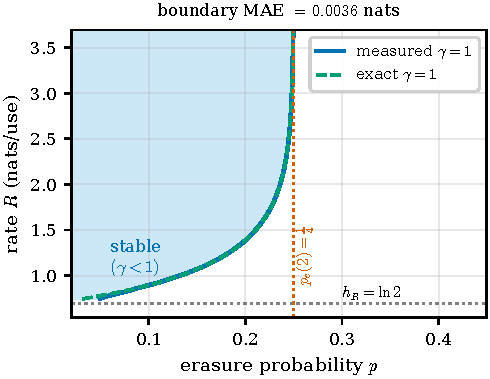
\includegraphics[width=\columnwidth]{fig_e4_phase.pdf}
\caption{The stability phase diagram for $m=2$ on the circle map. The measured $\gamma=1$ contour overlies the
exact analytic boundary to $0.0036$ nats. The stability region is the shaded area. The vertical asymptote at
$p_c(2)=1/4$ and the floor at the restoration entropy $\ln 2$ are the two marginals of the exact surface.}
\label{fig:phase}
\end{figure}

\subsection{Necessity, the reliability law, and why importance sampling is needed}
The reliability condition is a statement about rare bursts, so it cannot be checked by direct simulation.
Figure~\ref{fig:reliability} makes this concrete. In the left panel the importance-sampled multiplier lies
exactly on the analytic curve and crosses one at $p_c(2)=1/4$, while naive Monte Carlo underestimates it by one
to two orders of magnitude and would wrongly declare stability well past the threshold. In the right panel the
importance-sampled multipliers for the first, second, and fourth moments cross one at the parameter-free values
$k^{-m}$ equal to one half, one quarter, and one sixteenth. The measured crossings are $0.4954$, $0.2499$, and
$0.0625$ against the predicted $0.5$, $0.25$, and $0.0625$. Across three surrogates with rates $\ln 2$, $\ln 3$,
and $\ln\lambda_u$ and moment orders one through four, the law $\ln p_c(m)=-m r^\star$ holds with a mean
logarithmic error of $0.0017$, which Table~\ref{tab:scaling} records.

\begin{figure*}[t]
\centering
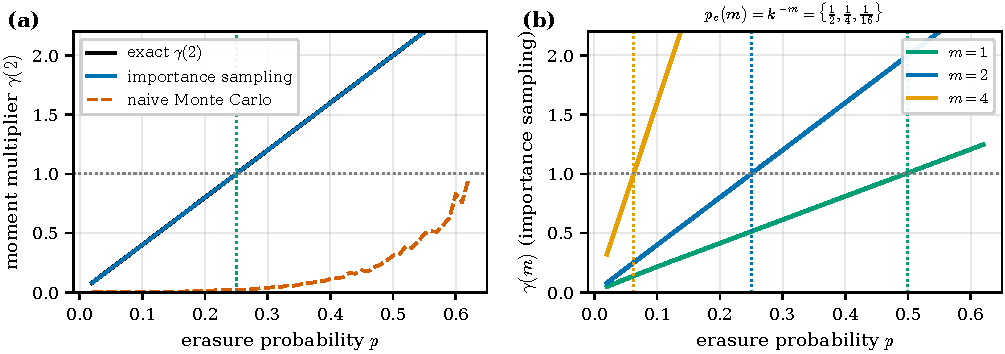
\includegraphics[width=\textwidth]{fig_e1_reliability.pdf}
\caption{The reliability threshold. (a) For $m=2$ the importance-sampled multiplier lies on the analytic curve
and crosses one at $p_c(2)=1/4$, while naive Monte Carlo is biased low by one to two orders of magnitude because
the moment is dominated by rare bursts. (b) The importance-sampled multipliers cross one at the parameter-free
thresholds $p_c(m)=k^{-m}$ for $m=1,2,4$.}
\label{fig:reliability}
\end{figure*}

\begin{table}[t]
\centering
\caption{The parameter-free reliability law $p_c(m)=e^{-m r^\star}$ across surrogates. Circle maps with tent and
doubling share the rate $\ln 2$ and give identical thresholds, so $p_c$ depends only on the rate.}
\label{tab:scaling}
\renewcommand{\arraystretch}{1.2}
\footnotesize
\begin{tabular}{@{}lcccc@{}}
\toprule
surrogate & $r^\star$ & $p_c(1)$ & $p_c(2)$ & $p_c(4)$ \\
\midrule
circle $k=2$, tent, doubling & $\ln 2$ & $0.4954$ & $0.2499$ & $0.0625$ \\
circle $k=3$ & $\ln 3$ & $0.333$ & $0.111$ & $0.0123$ \\
cat map & $\ln\lambda_u$ & $0.382$ & $0.146$ & $0.0213$ \\
\bottomrule
\end{tabular}
\end{table}

\subsection{The two conditions are independent}
At a finite rate the rate condition and the reliability condition appear as distinct transitions.
Figure~\ref{fig:conditions} shows this at rate $\ln 2 + 0.1$. The almost-sure escape rate, which is governed by
typical paths and by condition \eqref{eq:R}, transitions at $p_R=0.126$, while the moment multipliers, which are
governed by condition \eqref{eq:A}, cross one earlier and in the cascade $p_A(4)<p_A(2)<p_A(1)<p_R$ equal to
$0.0215$, $0.057$, $0.087$, and $0.126$. Higher moments are more fragile, and neither condition reduces to the
other. This also corrects a natural misreading, because at this finite rate the transition is not at the
high-rate marginal $1/4$ but at these exact values.

\begin{figure}[t]
\centering
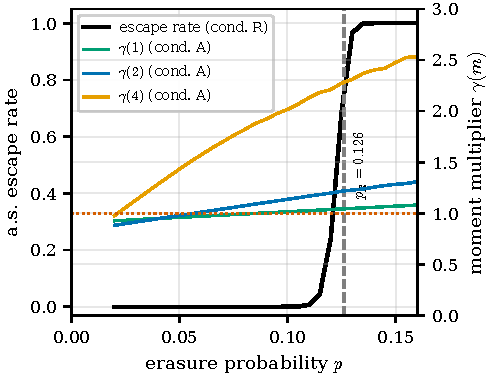
\includegraphics[width=\columnwidth]{fig_e2_two_conditions.pdf}
\caption{Two independent conditions at rate $\ln 2+0.1$. The almost-sure escape rate on the left axis transitions
at $p_R=0.126$, while the moment multipliers on the right axis cross one earlier, forming the cascade
$p_A(4)<p_A(2)<p_A(1)<p_R$. Neither condition reduces to the other.}
\label{fig:conditions}
\end{figure}

\subsection{The zooming quantizer reaches the threshold}
The achievability rests on a quantizer that keeps the encoder and decoder synchronized without acknowledgment.
Figure~\ref{fig:ach} confirms both its faithfulness and its sufficiency. In the left panel a genuine
two-dimensional cat-map observer, which iterates the true torus state and tracks a two-dimensional uncertainty
box, produces an escape curve indistinguishable from the reduced one-dimensional walk, with a mean absolute error
of $0.0001$, so zooming only along the unstable direction is exact. In the right panel the importance-sampled
second moment saturates and stays bounded when the multiplier is below one, at $\gamma=0.75$, and grows when it is
above one, at $\gamma=1.24$, which is the achievability and the necessity meeting at the exact surface.

\begin{figure*}[t]
\centering
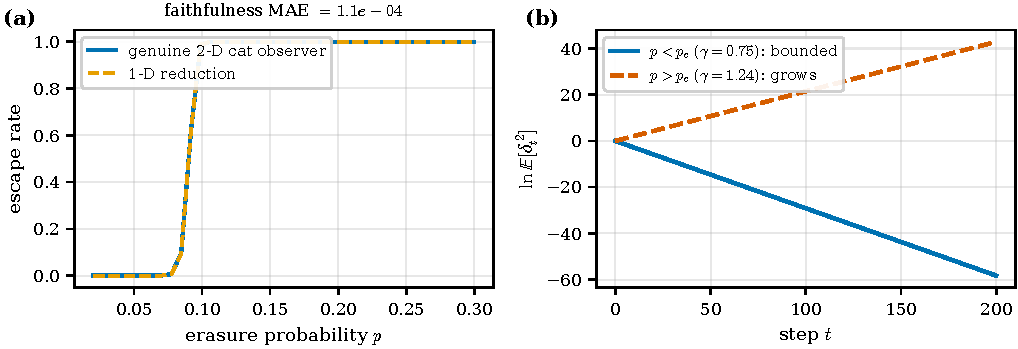
\includegraphics[width=\textwidth]{fig_e5_achievability.pdf}
\caption{The universal zooming quantizer. (a) A genuine two-dimensional cat-map observer matches the reduced
one-dimensional unstable-direction walk to a mean absolute error of $0.0001$. (b) The importance-sampled second
moment stays bounded for $\gamma=0.75$ below threshold and grows for $\gamma=1.24$ above threshold.}
\label{fig:ach}
\end{figure*}

\subsection{Two rates govern a vector plant}
The deepest prediction is that a plant with several unstable directions is governed by two different numbers, the
volume rate for bandwidth and the top rate for reliability. Figure~\ref{fig:tworate} tests this on a vector system
with volume rate $1.4$ and top rate $1.0$, which are genuinely different. In the left panel the almost-sure
escape under a proportional allocation, which budgets every mode, transitions at $p=0.329$, matching the volume
rate prediction $0.364$ and not the top rate prediction $0.545$, while an allocation that budgets only the
dominant mode escapes far earlier because the sub-dominant mode diverges. In the right panel the moment
multipliers cross one at the top rate thresholds, with the measured second-moment threshold $0.1352$ matching the
prediction $0.1353$. This separation cannot be seen on scalar surrogates, where the two rates coincide.

\begin{figure*}[t]
\centering
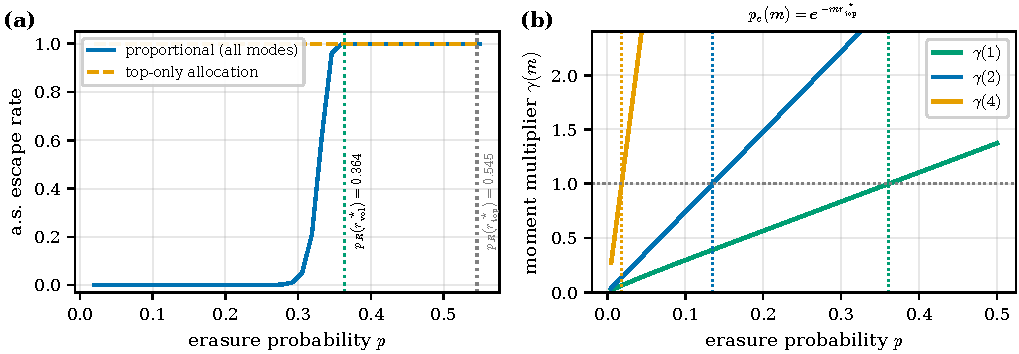
\includegraphics[width=\textwidth]{fig_m1_two_rates.pdf}
\caption{A vector plant with volume rate $1.4$ and top rate $1.0$. (a) The almost-sure escape under proportional
allocation binds on the volume rate, transitioning at $0.329$ against the prediction $0.364$, while a top-only
allocation escapes early. (b) The moment multipliers cross one at the top-rate thresholds, matching
$p_c(2)=0.1352$ against $0.1353$.}
\label{fig:tworate}
\end{figure*}

\subsection{Stress systems and correlated loss}
Three further tests probe the assumptions, and Table~\ref{tab:results2} summarizes the campaign. On non-normal
matrices, where the operator norm exceeds the spectral radius by up to a factor of $4.2$, the moment threshold is
the spectral-radius value $\rho(A)^{-m}$ to a mean absolute error of $0.0087$, and it is far from the naive
operator-norm value $\|A\|^{-m}$, whose error is $0.3011$, because long bursts self-average to the spectral radius
in the sense of Gelfand. Table~\ref{tab:nonnormal} lists these comparisons. On the non-uniform H\'enon map the
effective moment rate rises from the Lyapunov exponent $0.7255$ toward the worst-case value $1.3203$ as the moment
order grows, and the almost-sure escape follows the Lyapunov average at $0.5171$ against the prediction $0.5523$,
which is exactly why the worst-case restoration rate, not the average, is the right rate for moment guarantees. On
a Gilbert-Elliott channel with mean burst length ten, the observer loses track at a mean erasure of $0.0354$
against the i.i.d. value of $0.3959$, and the exact modulated moment-growth rate matches the spectral radius of
the modulated matrix to a mean absolute error of $0.0009$, which supports the correlated-loss conjecture and shows
that the i.i.d. threshold is a necessary but optimistic screen for bursty links.

\begin{table}[t]
\centering
\caption{Non-normal systems: the moment threshold is the spectral-radius value, not the operator-norm value.}
\label{tab:nonnormal}
\renewcommand{\arraystretch}{1.2}
\footnotesize
\begin{tabular}{@{}lcc@{}}
\toprule
prediction & MAE of $p_c$ & relative \\
\midrule
spectral radius $\rho(A)^{-m}$ & $0.0087$ & $1\times$ \\
operator norm $\|A\|^{-m}$ & $0.3011$ & $35\times$ \\
\bottomrule
\end{tabular}
\end{table}

\begin{table*}[t]
\centering
\caption{Summary of the experimental campaign. All errors in nats.}
\label{tab:results2}
\renewcommand{\arraystretch}{1.2}
\small
\begin{tabular}{@{}lll@{}}
\toprule
Experiment & Claim tested & Result \\
\midrule
Phase diagram & exact $\gamma=1$ surface & boundary MAE $0.0036$ \\
Reliability & $p_c(m)=e^{-m r^\star}$ via IS & $0.4954,0.2499,0.0625$ \\
Two conditions & (R) and (A) independent & $p_R=0.126$; cascade below \\
Achievability & zooming quantizer & faithfulness MAE $0.0001$ \\
Two rates & volume vs top rate & $0.329$ vs $0.364$; $0.135$ \\
Scaling law & across surrogates & mean log-error $0.0017$ \\
Universality & five maps & tent, doubling identical \\
Non-normal & spectral radius rate & $0.0087$ vs $0.3011$ \\
H\'enon & restoration vs Lyapunov & $r_{\rm eff}$ $0.725\!\to\!1.320$ \\
Gilbert-Elliott & bursts strictly worse & $0.035$ vs $0.396$ \\
\bottomrule
\end{tabular}
\end{table*}

%% ===========================================================================
\section{Discussion and Limitations}\label{sec:disc}
%% ===========================================================================
The exact result is proven for the memoryless erasure channel with uniformly hyperbolic surrogates, where the
restoration entropy equals the expansion rate and the threshold carries no estimation error. The correlated
Gilbert-Elliott channel is a separate generalization for which we give strong numerical evidence, namely that the
moment-growth rate is the spectral radius of a modulated matrix and that bursts are strictly more damaging than
i.i.d. loss at the same mean, but a first-principles proof for nonlinear maps under Markov loss remains open. The
achievability uses the exact multiplicative uncertainty recursion, which is faithful for these maps as the genuine
two-dimensional observer confirms, while the explicit no-acknowledgment anytime tree code is modelled by the
assumption that the index stream is eventually delivered, and its reliability requirement is exactly the erasure
tail that we validate. The non-uniform stress systems, whose restoration entropy has no closed form, are mechanism
validations rather than exact tests, and delay, which compounds the expansion, is left for future work. These
boundaries are consistent with the numbers above and mark the natural extensions.

%% ===========================================================================
\section{Conclusion}\label{sec:conc}
%% ===========================================================================
We have determined the exact $m$-th-moment threshold for controlling a general expansive nonlinear system over a
memoryless erasure channel. The error is bounded if and only if a single per-step multiplier is below one, and the
two edges of this surface are a bandwidth requirement set by the restoration entropy and a reliability requirement
set by the top expansion rate. A universal zooming quantizer reaches the exact threshold with no
quasi-conformality assumption, so necessity and sufficiency meet with no gap, and a plant with several unstable
directions is governed by two different rates. Rare-event importance sampling confirms every prediction to within
a few thousandths of a nat. The practical message is that guaranteeing average throughput alone is not enough for
an unstable workload, because survival also requires enough burst reliability to ride out runs of lost packets.
Natural next steps are a proof of the correlated-loss threshold, an explicit anytime code, and the delay-augmented
threshold.

%% ===========================================================================
\bibliographystyle{IEEEtran}
\bibliography{../References/refs}

\end{document}
